\documentclass[conference,12pt]{IEEEtran}

\usepackage[tight,footnotesize]{subfigure}

\usepackage[pdftex]{graphicx}
\graphicspath{{./images/}}

\hyphenation{op-tical net-works semi-conduc-tor}

\begin{document}
	
\title{\vspace{-0.05\textheight}System Design Project - Report 3}

\author{\vspace{-0.05\textheight}\IEEEauthorblockN{Marc Howarth}
\IEEEauthorblockA{Group 12 - Robot Unicorn Defenders}}
	
\maketitle

\IEEEpeerreviewmaketitle

\section{Introduction}
MEXICAN HAT DANCE!!!
	
\section{GUI}
A critical part of being able to test our robot has been the ability to select different options easily on the GUI. Figure \ref{fig:GUI} shows all the different choices that we can choose from:
\begin{itemize}
 \item \textit{Goal}: Choose the goal that we are aiming at.
 \item \textit{Our Robot}: Determines if our robot is mounted with the blue or yellow plate.
 \item \textit{Processor}: Get the location information from either a file, a process (i.e. our vision system) or a simulator.
 \item \textit{Strategy}: A list of strategies including goToBall and takePenalty.
 \item \textit{Executor}: Exectue the commands on the simulator or through Bluetooth.
\end{itemize}
Most of the GUI was implemented by Joe however, I realised, after testing the robot that we would need the ability to choose which goal is ours, and which is our opponents. This led to some flaws in our strategies that had assumed a single goal position, but were quickly updated.

\section{Sensors}
One of the construction team's iterations included a light sensor placed behind the kicker. I decided to try and utilise the sensor within the code on the brick. This required a lot of calibration because the lighting levels in different rooms changed the values of high and low level of light. To get around this, I create a program that calibrated the light levels and outputted the required parameters.

We used the light sensor to determine when the ball was infront of it, however it could have also been used to know wether the robot was about to run into a wall or any obstacle. The light sensor emits a red light which may effect other teams vision, so, after speaking to Garry, we may still be able to use the sensor but there's no definite way of knowing until we try. Because of this we decided to not use a light sensor and include two touch snesors instead.

\section{GoToBall}


\section{Moments}


\section{Testing}


\pagebreak

\section{Appendix}
\begin{figure}[htp]
\begin{center}
\leavevmode
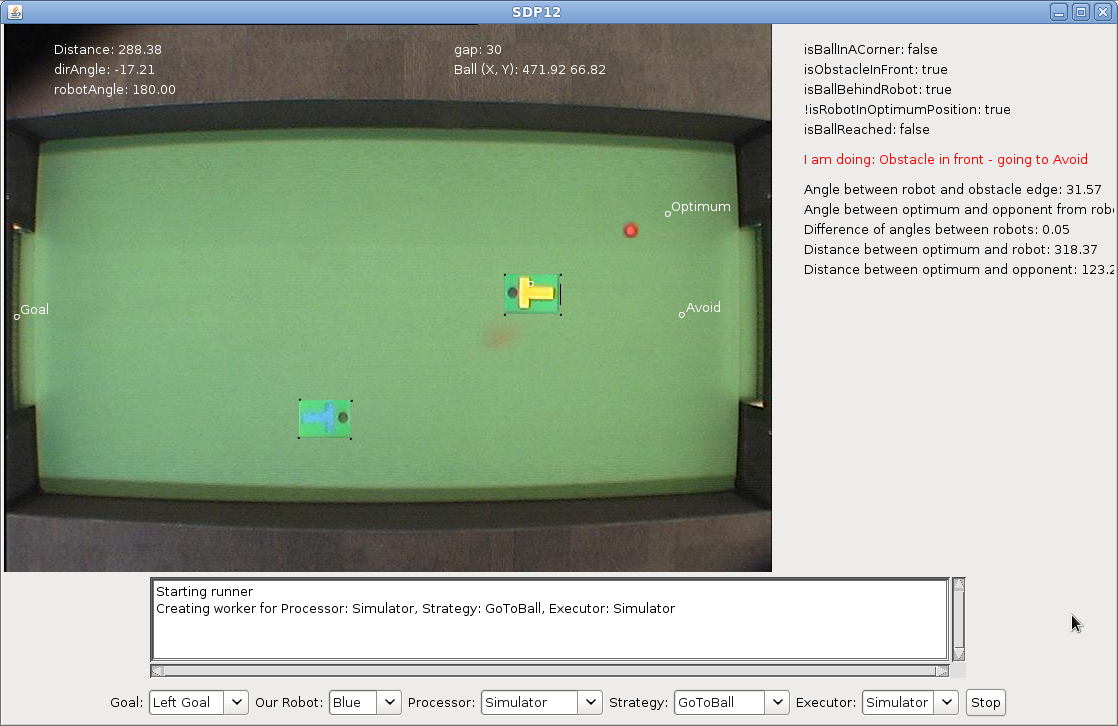
\includegraphics[width=0.8\textwidth] {GUI.png}
\end{center}
\caption{Screenshot of GUI running the simulator}
\label{fig:GUI}
\end{figure}

\end{document}
